%%%%%%%%%%%%%%%%%%%%%%%%%%%%%%%%%%%
%This is the LaTeX COMMUNICATION template for RSC journals
%Copyright The Royal Society of Chemistry 2016
%%%%%%%%%%%%%%%%%%%%%%%%%%%%%%%%%%%

\documentclass[twoside,twocolumn,9pt]{article}
\usepackage{extsizes}
\usepackage[super,sort&compress,comma]{natbib} 
\usepackage[version=3]{mhchem}
\usepackage[left=1.5cm, right=1.5cm, top=1.785cm, bottom=2.0cm]{geometry}
\usepackage{balance}
\usepackage{comment}
\usepackage{mathptmx}
\usepackage{sectsty}
\usepackage{graphicx} 
\usepackage{lastpage}
\usepackage[format=plain,justification=justified,singlelinecheck=false,font={stretch=1.125,small,sf},labelfont=bf,labelsep=space]{caption}
\usepackage{float}
\usepackage{fancyhdr}
\usepackage{fnpos}
\usepackage[english]{babel}
\addto{\captionsenglish}{%
  \renewcommand{\refname}{Notes and references}
}
\usepackage{array}
\usepackage{droidsans}
\usepackage{charter}
\usepackage[T1]{fontenc}
\usepackage[usenames,dvipsnames]{xcolor}
\usepackage{setspace}
\usepackage[compact]{titlesec}
\usepackage{hyperref}
\usepackage[capitalize,noabbrev]{cleveref}
%%%Please don't disable any packages in the preamble, as this may cause the template to display incorrectly.%%%


\usepackage{epstopdf}%This line makes .eps figures into .pdf - please comment out if not required.

\definecolor{cream}{RGB}{222,217,201}
%%%%%%%%% Preamble of the bibliography, can be commented or deleted 
\def\bibpreamble{}
%%%%%%%%% 
\begin{document}

\pagestyle{fancy}
\thispagestyle{plain}
\fancypagestyle{plain}{
%%%HEADER%%%
\renewcommand{\headrulewidth}{0pt}
}
%%%END OF HEADER%%%

%%%PAGE SETUP - Please do not change any commands within this section%%%
\makeFNbottom
\makeatletter
\renewcommand\LARGE{\@setfontsize\LARGE{15pt}{17}}
\renewcommand\Large{\@setfontsize\Large{12pt}{14}}
\renewcommand\large{\@setfontsize\large{10pt}{12}}
\renewcommand\footnotesize{\@setfontsize\footnotesize{7pt}{10}}
\renewcommand\scriptsize{\@setfontsize\scriptsize{7pt}{7}}
\makeatother

\renewcommand{\thefootnote}{\fnsymbol{footnote}}
\renewcommand\footnoterule{\vspace*{1pt}% 
\color{cream}\hrule width 3.5in height 0.4pt \color{black} \vspace*{5pt}} 
\setcounter{secnumdepth}{5}

\makeatletter 
\renewcommand\@biblabel[1]{#1}            
\renewcommand\@makefntext[1]% 
{\noindent\makebox[0pt][r]{\@thefnmark\,}#1}
\makeatother 
\renewcommand{\figurename}{\small{Fig.}~}
\sectionfont{\sffamily\Large}
\subsectionfont{\normalsize}
\subsubsectionfont{\bf}
\setstretch{1.125} %In particular, please do not alter this line.
\setlength{\skip\footins}{0.8cm}
\setlength{\footnotesep}{0.25cm}
\setlength{\jot}{10pt}
\titlespacing*{\section}{0pt}{4pt}{4pt}
\titlespacing*{\subsection}{0pt}{15pt}{1pt}
%%%END OF PAGE SETUP%%%

%%%FOOTER%%%
\fancyfoot{}
\fancyfoot[LO,RE]{\vspace{-7.1pt}\includegraphics[height=9pt]{head_foot/LF}}
\fancyfoot[CO]{\vspace{-7.1pt}\hspace{13.2cm}\includegraphics{head_foot/RF}}
\fancyfoot[CE]{\vspace{-7.2pt}\hspace{-14.2cm}\includegraphics{head_foot/RF}}
\fancyfoot[RO]{\footnotesize{\sffamily{1--\pageref{LastPage} ~\textbar  \hspace{2pt}\thepage}}}
\fancyfoot[LE]{\footnotesize{\sffamily{\thepage~\textbar\hspace{3.45cm} 1--\pageref{LastPage}}}}
\fancyhead{}
\renewcommand{\headrulewidth}{0pt} 
\renewcommand{\footrulewidth}{0pt}
\setlength{\arrayrulewidth}{1pt}
\setlength{\columnsep}{6.5mm}
\setlength\bibsep{1pt}
%%%END OF FOOTER%%%

%%%FIGURE SETUP - please do not change any commands within this section%%%
\makeatletter 
\newlength{\figrulesep} 
\setlength{\figrulesep}{0.5\textfloatsep} 

\newcommand{\topfigrule}{\vspace*{-1pt}% 
\noindent{\color{cream}\rule[-\figrulesep]{\columnwidth}{1.5pt}} }

\newcommand{\botfigrule}{\vspace*{-2pt}% 
\noindent{\color{cream}\rule[\figrulesep]{\columnwidth}{1.5pt}} }

\newcommand{\dblfigrule}{\vspace*{-1pt}% 
\noindent{\color{cream}\rule[-\figrulesep]{\textwidth}{1.5pt}} }

\makeatother
%%%END OF FIGURE SETUP%%%

%%%TITLE AND AUTHORS%%%
\twocolumn[
  \begin{@twocolumnfalse}
{\includegraphics[height=30pt]{head_foot/journal_name}\hfill\raisebox{0pt}[0pt][0pt]{\includegraphics[height=55pt]{head_foot/RSC_LOGO_CMYK}}\\[1ex]
\includegraphics[width=18.5cm]{head_foot/header_bar}}\par
\vspace{1em}
\sffamily
\begin{tabular}{m{4.5cm} p{13.5cm} }

\includegraphics{head_foot/DOI} & \noindent\LARGE{\textbf{Assessing coding-agent reliability in molecular dynamics workflows with MDArena}} \\% Original title: Tracking the capabilities and limits of AI Agents in MD workflows with MDArena
 & \vspace{0.3cm} \\

 & \noindent\large{Nithishwer Mouroug Anand\textit{$^{a\ast\ddag}$},
Wei-Tse Hsu\textit{$^{a\ddag}$}, Kyle Vaccaro\textit{$^{a,b}$},
Eden James Gage\textit{$^{a}$}, Jonathan David Colburn\textit{$^{a}$},
Linda Xi Phan\textit{$^{a}$}, Minjoon Seo\textit{$^{a}$},
Kevin Guan\textit{$^{a}$} and Philip C. Biggin\textit{$^{a\ast}$}} \\

\includegraphics{head_foot/dates} &
\noindent\normalsize{

Abstract to be added.
%%%ABSTRACT%%%%


% \textbf{Might Need refining based on Discussion and Conclusions}

% {\sffamily\bfseries Coding agents increasingly automate scientific workflows, but their reliability in molecular dynamics (MD) research remains unclear. In this article we evaluate LLM based frontier coding agents on  MDArena, a benchmark of 50 containerized tasks drawn from active biomolecular simulation projects, spanning 29 molecular systems and 14 broad research protocols and identify the limits and cabailities and reliability of these agents. We show that LLM Based agents have reached production level of reliability and can be confiderently used in tasks without much human supervison. We evaluate 12+ model–harness configurations across Codex, Claude Code, and OpenCode, with three attempts per task on 50 tasks, for a total of 1,800 trials. Claude Code–Opus-5.5 achieved the highest Strict-Pass@1 rate at 94.7\% (142/150 trials),  followed by Codex–GPT-6.1 Sol and Codex–GPT-6 Astra, both at 88.0\% (132/150 each). Mean correctness and process scores exceeded strict pass rates for every configuration, showing that agents often met some requirements without satisfying all checks. Across the 16 hard tasks, Claude Code–Opus-5.5 led at 91.7\% (44/48 trials), up from 52.1\% (25/48) for Claude Code–Opus-5, while OpenCode–Gemini 4 Argon ranked second at 81.3\% (39/48). These gains show that newer agents can complete many demanding molecular dynamics workflows, while the remaining failures underscore the value of independent validation. MDArena provides a reproducible and extensible platform for tracking both progress and persistent failures.}


%%%END OF ABSTRACT%%%%
} \\

\end{tabular}

 \end{@twocolumnfalse} \vspace{0.6cm}

  ]
%%%END OF TITLE AND AUTHORS%%%

%%%FONT SETUP - please do not change any commands within this section
\renewcommand*\rmdefault{bch}\normalfont\upshape
\rmfamily
\section*{}
\vspace{-1cm}


%%%FOOTNOTES%%%

\footnotetext{\textit{$^{a}$~University of Oxford. E-mail: nithishwer.mourouganand@reuben.ox.ac.uk; philip.biggin@bioch.ox.ac.uk}}
\footnotetext{\textit{$^{b}$~Scripps Research Institute.}}

%Please use \dag to cite the ESI in the main text of the article.
%If you article does not have ESI please remove the the \dag symbol from the title and the footnotetext below.
%\footnotetext{\dag~Supplementary Information available: [details of any supplementary information available should be included here]. See DOI: 00.0000/00000000.}
%additional addresses can be cited as above using the lower-case letters, c, d, e... If all authors are from the same address, no letter is required

\footnotetext{\ddag~Nithishwer Mouroug Anand and Wei-Tse Hsu contributed equally to this work.}
\footnotetext{$\ast$~Corresponding authors: Nithishwer Mouroug Anand and Philip C. Biggin.}

%%%END OF FOOTNOTES%%%

% Overall comments
\begin{comment}
    - As mentioned previously, I think one of the most important thing to add in the discussion is the current challenge of creating difficult, realistic, and benchmarkable tasks for AI agents.
      - Making scientific work reliably benchmarkable can remove some of the decisions that made it scientifically difficult. The challenge is to preserve meaningful scientific judgment while keeping evaluation fair and credible.  Specifying a task can give away its intellectual content.
      - Human difficulty does not necessarily predict agent difficulty. (AI agents is good at procedural problems.)
      - The difficulty ceiling of MDArena does not reflect the difficulty ceiling of research. Agents can perform many technically demanding components of MD research when the scientific objective, available inputs, and deliverables are sufficiently defined.
    - We should probably tone down statements like "reached production level of reliability", "confidently used ... without much human supervision", "ready for adoption in production workflow". The benchmark establishes performance on 50 bounded tasks in prepared envs under specified resource limits. It does not establish reliability on unseen projects, open-ended research, or downstream scientific conclusions. 
    - One thing we could emphasize is that a small number of failed checks does not imply a small scientific error. 
    - Observations
      - Similar aggregate success can conceal different efficiency (sol and astra both at 88%, with substantially different costs)
      - Distinction between recognizing a problem and acting on that recognition. Your TB-Science experience suggests this distinction; MDArena’s Task 39 potentially supplies its own evidence through agents acknowledging charge-treatment concerns but leaving them unresolved. If supported by the trajectories, that is a stronger observation than “agents lack domain knowledge”: they may articulate relevant knowledge yet fail to incorporate it into the delivered workflow.
    - From AI: The draft’s progression from earlier scores to current scores is attractive, but the repository records changes to inputs, reference answers, correctness checks, and process-judge access. A dagger identifying an older dataset version does not make those measurements comparable.
    Before making “improvement from 52.1% to 91.7%” a central claim, establish whether both configurations were evaluated under equivalent task and grading conditions. If not:
        - Make the current evaluation the main result.
        - Present older evaluations as historical context, explicitly separated.
        - Avoid attributing the entire difference to model improvement.
        There is no need to rerun every historical model simply to retain a timeline.
    - Paragraphs to consider
      - The high success rates observed here suggest that technical complexity and human effort do not necessarily confer lasting difficulty for coding agents. Research-derived workflows can require substantial expertise while becoming tractable once their objectives, inputs, and expected outputs are defined. MDArena’s approaching performance ceiling therefore limits its ability to distinguish the strongest configurations, while documenting their capacity to execute a substantial range of bounded molecular dynamics tasks. These results do not establish equivalent proficiency in formulating scientific questions, selecting appropriate investigations, or determining whether the resulting evidence is sufficient.
      - Extending scientific benchmarks involves a tension between preserving scientific judgment and enabling reliable evaluation. Instructions that prescribe methods, controls, and diagnostic steps can remove decisions that the evaluation intends to test. Conversely, underspecified tasks can admit multiple defensible solutions that narrow verifiers reject. Future extensions should distinguish clear scientific requirements from solution steps that agents must discover, accept scientifically valid alternative approaches, and assess the consequences of errors rather than pursuing low success rates alone. Increasing computational expense or adding constraints does not necessarily improve the measurement of scientific capability.
      - As agents become more proficient at implementing molecular simulation workflows, expert oversight may increasingly concentrate on defining scientific requirements and verifying that final artifacts preserve them.
      - MDArena measures whether an attempt passes. A separate, practically important question is whether the agent recognizes when its own output is unreliable.\
        - Your existing final answers and trajectories could support a small supplementary analysis:
            - Did the agent claim successful completion?
            - Did it disclose the defect that caused failure?
            - Did it distinguish completed work from unresolved work?
      - Strict success measures satisfaction of the complete task specification; differences between tasks therefore reflect both their scientific demands and the scope of the required deliverables.
      - An informative analysis would ask: How often does process grading reject an otherwise correctness-passing attempt, and what does it catch? The reverse comparison is useful too.
      Explicit instructions can improve reliable delegation. But if a scientist must specify every diagnostic, control, and methodological decision, the agent is contributing primarily implementation effort. Neither outcome is undesirable. They simply represent different levels of assistance. This suggests a useful distinction for the paper:
        - Delegation: execute a scientifically specified workflow.
        - Scientific assistance: help identify the appropriate workflow and necessary checks.
        - Independent investigation: determine which questions and evidence should guide subsequent work.
        MDArena spans parts of the first two. Its results should not be generalized to the third.
    - TODOS
        - Introduction: Check recent literature to include
        - Ask GPT to see if there are any references missing. Scan the repo as well. 
        - Unify the bib style.
        
\end{comment}


\rmfamily %Please do not remove this line.

%%%MAIN TEXT%%%%


\section{Introduction}

Molecular dynamics (MD) has become central to modern biomolecular research.\cite{hollingsworth2018molecular,huggins2019biomolecular} While its theoretical foundation is well-established, carrying out a scientifically reliable MD workflow remains technically demanding, as it often requires substantial expertise for meticulous system preparation, parameterization, selection of sampling protocols, and analysis tailored to the scientific question. Powered by large language models (LLMs)\cite{zhao2023survey} and equipped to directly interact with computational environments, coding agents\cite{liu2024large} offer a promising route to automate substantial portions of this work. 

On this front, several studies have demonstrated this potential across increasingly sophisticated workflows. For biomolecular applications, MDCrow\cite{campbell2026mdcrow} introduced an LLM-based assistant for routine protein MD tasks, while NAMD-Agent\cite{chandrasekhar2025namdagent} and DynaMate \cite{guilbert2025dynamate} automated protein and protein–-ligand simulation and analysis through specialized pipelines. In materials simulation, PolyJarvis\cite{zhao2026polyjarvis} and LAMMPS-Agents\cite{vriza2026multiagentic} enabled end-to-end LAMMPS\cite{thompson2022lammps} workflows for predicting properties of polymers and inorganic materials, respectively, while ChemGraph\cite{pham2026chemgraph} presents agentic tool orchestration for general computational-chemistry problems. Recently, dedicated benchmarks MD-EvalBench\cite{shi2026mdagent2} and MDGym\cite{kumar2026mdgym} have also been proposed, which evaluate coding agents on executable tasks using LAMMPS\cite{thompson2022lammps} and GROMACS.\cite{abraham2015gromacs} 

While these efforts establish the feasibility of agentic molecular simulation, existing evaluations remain limited in their ability to represent the breadth and complexity of computational chemistry research. Specifically, they typically either assess purpose-built agents on small sets of isolated or simplified cases, or comprise repeated variations of the same general workflow, such as setting up simulations to compute specified properties.\cite{kumar2026mdgym} It therefore remains unclear whether general-purpose coding agents can reliably tackle heterogeneous, long-horizon problems common in actual research projects and drug-discovery campaigns. Beyond test coverage, their emphasis on execution success or agreement with a reference output also provides limited support for assessing workflow validity, as a flawed system or inappropriate protocol may still execute successfully and produce plausible results. Given the rapid improvement of the LLMs underlying coding agents, realistic benchmarks are urgently needed to identify their capabilities and limitations. In particular, analysis of repeated runs and individual failures can further establish how consistently agents complete research tasks and where independent validation remains necessary.

We therefore introduce MDArena, an executable benchmark of 50 expert-curated, containerized tasks drawn directly from actual research projects in biomolecular simulations. Characterized by three difficulty levels, the benchmark tasks span 29 diverse biomolecular systems and 18 simulation software packages, covering tasks including membrane-protein preparation, parameterization of non-standard residues, free energy methods, enhanced-sampling protocols, quantum-chemistry workflows, and bespoke analysis across diverse research contexts (see Figures \ref{fgr:task-types} and \ref{fig:representative_tasks}).

\begin{figure}[h]
\centering
  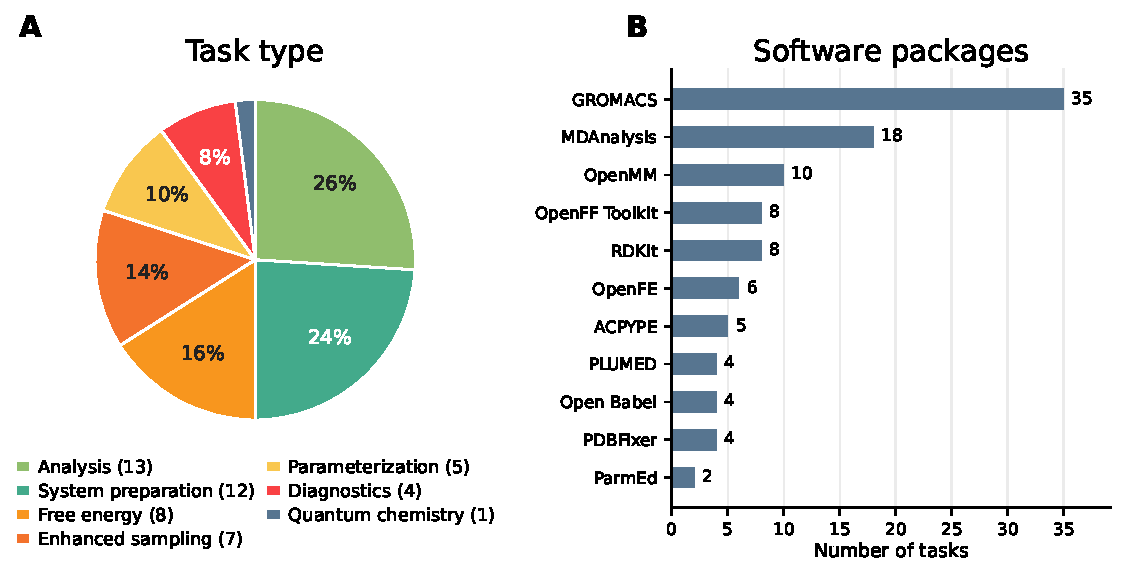
\includegraphics[width=\columnwidth]{figures/figure_1/figure_1.pdf}
  \caption{Composition of the 50 MDArena tasks by (A) task type and (B) software package. Each task has one task type and may use multiple packages. Panel B shows packages used in at least two tasks.}
  \label{fgr:task-types}
\end{figure} 

Each task is implemented using Harbor,\cite{Harbor_Framework}, an established agent evaluation framework supporting benchmarks such as Terminal-Bench 2.0\cite{merrill2026terminal}, SWE-bench Verified\cite{chowdhury2024swebenchverified}, and Terminal-Bench-Science\cite{terminal2026terminal}. This setup makes it straightforward to evaluate new agents and incorporate new research problems, allowing MDAren to evolve with the frontiers of computational chemistry research and remain informative as agent capabilities advance. In MDArena, each task is evaluated by deterministic checks of the submitted artifacts and LLM-based assessment of the workflow’s scientific validity to distinguish sound solutions from merely plausible outputs. Using MDArena, we evaluate 18 contemporary model–harness configurations released between May and November 2026 under a common execution protocol and this two-part verification scheme. The evaluation assesses strict task success, partial-credit scores, repeatability, computational cost, and observed failure modes.

Across these evaluations, the strongest agents successfully completed a broad range of demanding MD tasks, from trajectory analysis to complex membrane-protein free energy setup. Claude Opus-5.5 achieved the highest strict pass rate at 94.7\% (142 of 150 trials), while GPT-6.1 Sol was the most cost-effective configuration, with an 88.0\% strict pass rate (132 of 150 trials) and a cost of \$0.53 per strict pass, compared with \$0.91 for Opus-5.5. Gemini-4 Argon and open-source models such as GLM also performed competitively. Nevertheless, individual failures across models included invalid final system assemblies, unresolved scientific requirements, and incomplete delivery within the allotted time. Together, these results characterize the state of the art in agentic assistance for bounded, reserach-derived molecular dynamics workflows while identifying specific points where independent validation remains necessary.

\begin{figure*}[t]
\centering
  \includegraphics[width=\textwidth]{figures/figure_2/figure_2.png}
  \caption{Representative tasks and systems in MDArena. Tasks in MDArena are diverse in both systems and problems of interest. Representative tasks include (A) planning a relative binding free-energy network for GPCR ligands using OpenFE~\cite{openfe} (Task 33), (B) constructing a PepT2-amoxicillin QM cluster for  proton-transfer scan in ORCA~\cite{neese2020orca} (Task 38), (C) extending CHARMM36~\cite{huang2013charmm36} to parameterize a pAsp-containing peptide (Task 47), and (D) performing alchemical metadynamics~\cite{hsu2023alchemical} to estimate absolute binding free energy of a host-guest complex (Task 48). Descriptions of these tasks and more can be found in the Supporting Information.}
  \label{fig:representative_tasks}
\end{figure*}

\section{Methods}

\subsection{Task selection and curation}

MDArena was constructed from more than 100 candidate tasks contributed by domain experts to reflect the diversity and difficulty of problems encountered in research projects and drug discovery efforts. The associated systems, trajectories, and intermediate files were drawn from completed or ongoing research projects~\cite{huang2013charmm36,jo2008charmm,kaminski2001evaluation,lindorff2010improved,hsu2023alchemical,dore2011structure,gerstenberger2020discovery,vojtvechovsky1999crystal,joshi2026structural,yin2015crystal,suno2018crystal,liu2012structural,hsu2022identifying,christopher2015fragment,chien2010structure,parker2024structural,hsu2024replica,borodovsky2020small}. We screened the candidates for scientific relevance, technical substance, and complementarity, yielding an initial release of 50 tasks. The collection deliberately includes long-horizon workflows, underspecified problems requiring scientific judgements, and negative examples where the requested action is impossible or scientifically inappropriate. 

The resulting benchmark spans 7 task types, 29 unique systems in 5 system types, and 18 software packages~\cite{abraham2015gromacs,eastman2024openmm,beckstein2016mdanalysis,case2023ambertools,sousa2012acpype,boothroyd2023development,landrum2013rdkit,o2011open,openfe,wu2024alchemlyb,tribello2014plumed,neese2020orca,merz2018testing,merz2022physical_validation}. Its aggregate composition is shown in Figure 1, with complete task-level metadata provided in Table S1. Each task was assigned an easy, medium, or hard difficulty label by the task author and subsequently reviewed based on the workflow length, required domain knowledge, and technical complexity. The current benchmark comprises 10 easy, 24 medium and 16 hard tasks. 

\subsection{Implementation}

MDArena is implemented using the Harbor\cite{Harbor_Framework} evaluation framework, allowing researchers to readily evaluate their own agents and extend MDArena with new self-contained tasks. Each task runs in a dedicated Docker container\cite{moreau2023containers} and includes an executable reference solution that passes all correctness and process checks, confirming task solvability and validating that the verifier functions as intended. Command-line interfaces are provided for analyzing evaluation runs and collecting portable run records. 

To facilitate reproducibility and robustness, MDArena implements several safeguards. Task-content digests and run-metadata validation support checks of dataset integrity and evaluation configuration. Canary strings are embedded in task instructions, configuration files, verifiers, and reference-solution scripts to identify benchmark material and support the exclusion of our benchmark from future model-training corpora. Lastly, we implement continuous integration to run unit and regression tests for evaluation tools and task-specific verifiers, validate task structure, and check verifier dependencies in a containerized environment. 

\subsection{Verification}

As molecular simulations are inherently stochastic and often lack a unique ground truth,\cite{wan2021uncertainty,communicationsbiology2023checklist}  MDArena primarily focuses on stages such as system preparation, simulation configuration, and post-simulation analysis, where in fact much of the technical difficulty of an MD workflow lies and where outputs can often be evaluated deterministically. Each executed task is evaluated by a two-part verifier that combines deterministic correctness checks with LLM-based process assessment. 

Specifically, deterministic correctness checks examine whether the resulting artifacts satisfy task-specific numerical, structural, and software-level requirements. They include scored checks that assess artifact content, as well as sanity checks that carry no correctness weight, such as file-existence checks. Where appropriate, verification independently reconstructs preparation steps or inspects compiled simulation inputs and accommodates scientifically valid alternatives without requiring exact reproduction of the reference solution. All correctness checks have been validated through Oracle sweeps, which execute the reference solutions and check for full correctness scores, as well as Nop sweeps, which check that performing no operation receives zero correctness credit. These sweeps are complemented by targeted regression tests using valid and invalid artifacts. 

Complementing the artifact-based deterministic checks, the process checks use an LLM judge to assess the agent’s execution trajectory against predefined criteria covering the scientific decisions and interpretations necessary for a valid solution. The corresponding correctness and process scores are computed as the weighted fractions of criteria satisfied. Together, these two scores distinguish valid solutions from superficially convincing workflows and reveal cases in which a sound process nevertheless produces an incorrect result. 

\subsection{Experimental setup}

We tracked the performance of frontier models from May 2026 onwards (see Figure~\ref{fig:model_performance}A), covering both open-source and proprietary models from OpenAI (GPT-5.5 Medium and XHigh, GPT-5.6 Sol and Terra, GPT-6.1 Sol, and GPT Astra), Anthropic (Claude Opus-5, Opus-5.5, and Sonnet-5), Google (Gemini Flash 3.5, Pro 3.1, 3.7 Flash, and 4 Argon), DeepSeek (V3.2), Alibaba (Qwen3-235B and Qwen3 Coder 480B A35B), and Z.ai (GLM-5.2). Across these 18 model--harness configurations, we conducted 2100 trials in total. Twelve configurations were evaluated with three independent replicates per task across all 50 tasks, contributing 1800 trials and forming the basis of our primary comparisons. The remaining six configurations were GPT-5.5 Medium and XHigh, Gemini 3.5 Flash, Gemini 3.1 Pro Preview, DeepSeek V3.2, and Qwen 3 Instruct 235B A22B. These earlier-generation configuratoins were evaluated with one replicate per task on MDArena v0.1, contributing 300 trials included in Figure~\ref{fig:model_performance} for historical context. 

Among the twelve configurations evaluated with three replicates, seven were evaluated on MDArena v0.2 and five on v1.0 (see Figure~\ref{fig:model_performance}). To ensure consistent scoring across these two batches, we manually reviewed changes to the task definitions and verification criteria. Where criteria were revised to accommodate scientifically valid solutions, we checked whether the revisions affected the earlier evaluations, and regraded affected trials where necessary. The reported results have incorporated these corrections to make the two batches directly comparable. Claude Opus-5 was used as the process judge all the three-replicate evaluations, while the historical v0.1 evaluations used Claude Opus-4.8.

In MDArena, tasks were executed in Docker containers with internet access, with GitHub and repository mirrors blocked to prevent task lookup. Each task had access to 2–-4 CPUs, 8 GB RAM, 10 GB storage, no GPUs, and a task-specific wall-clock limit ranging from 10 minutes to 2.5 hours given its computational requirements. 

\subsection{Evaluation metrics and statistical analysis}

For each configuration, the reported strict-pass@1 rate was calculated as the fraction of individual trials that pass all scored correctness and process checks:
\begin{equation}
\mathrm{Strict\mbox{-}Pass@1}
= \frac{1}{NR}\sum_{i=1}^{N}\sum_{r=1}^{R}s_{ir},
\end{equation}
where $N$ is the number of tasks, $R$ is the number of replicates per task, and $s_{ir}$ equals one if replicate $r$ on task $i$ achieves a strict pass and zero otherwise. Mean correctness and process scores were calculated by averaging the corresponding scores across all trials. For configurations evaluated with three replicates per task, Pass@3 denotes the fraction of tasks with at least one strict pass, while Pass$^3$ as a repeatability measure denotes the fraction with strict passes in all three replicates.

Timeouts and other runtime failures were retained as failed deliveries and assigned zero correctness and process scores in the adjusted metrics. Confidence intervals were computed as 95\% percentile bootstrap intervals from 2000 resamples, sampling tasks rather than trials so that repeated attempts at one task were not treated as independent.

\section{Results and discussion}

% Queue the full-width figure early so it can appear with the results.
\begin{figure*}[t]
\centering
  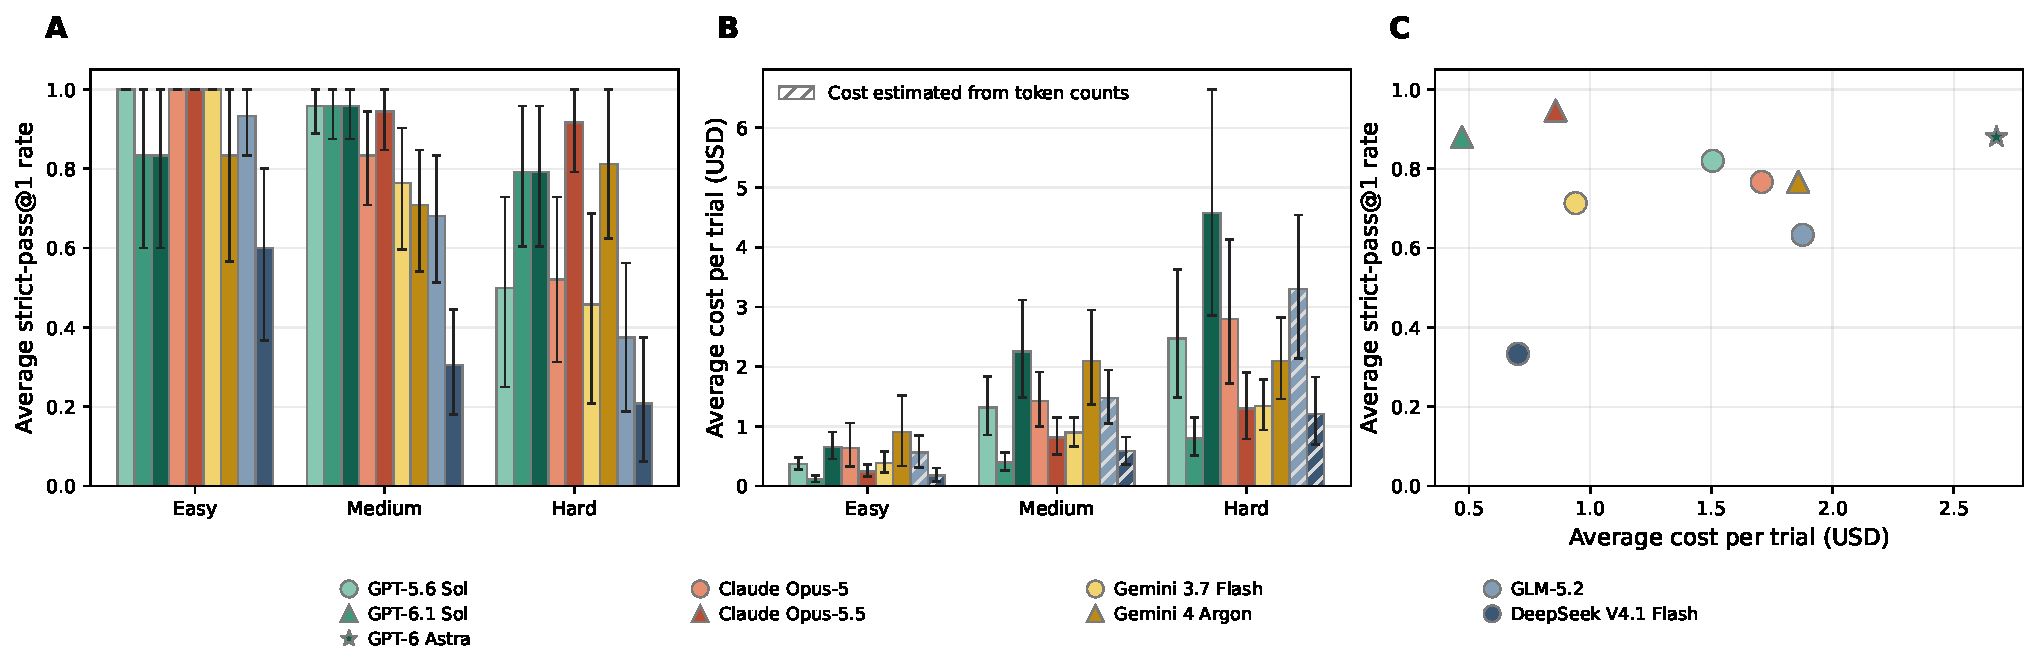
\includegraphics[width=\textwidth]{figures/figure_3/figure_3.pdf}
  \caption{Performance of the evaluated coding agents on MDArena. (A) Mean Strict-Pass@1 against model release date. (B, C) Mean correctness and process scores, respectively, for five selected models. Error bars show 95\% task-bootstrap confidence intervals. Superscript stars ($\ast$) mark v0.2 runs with three attempts per task; daggers ($\dagger$) mark historical v0.1 runs with one attempt per task. Unmarked configurations use v1.0 with three attempts per task. Historical evaluations provide context for progress and differ from the repeated evaluations in benchmark version and grading protocol.}
  \label{fig:model_performance}
  \label{fig:success-reward-triptych}
\end{figure*}


\subsection{Frontier agents complete increasingly demanding MD workflows across diverse research tasks}
% This subsection combines the original subsections 3.1 and 3.3
% \subsection{Frontier coding agents can reliably execute complex molecular dynamics workflows}  % 3.1
% \subsection{Frontier models tested solve previously intractable hard tasks}  % 3.3

Frontier LLMs have made a leap in capabilities over the past few months, and this is reflected in their MDArena scores (Figure~\ref{fig:model_performance}). In the initial v0.1 evaluation, Gemini 3.1 Pro Preview and  GPT-5.5 with extra-high reasoning effort achieved strict pass rates of 34\% and 48\%, respectively. The latest frontier models, however, perform substantially better: Gemini 4 Argon achieved 76.7\%, GPT-6.1 Sol and GPT-6 each achieved 88.0\%, while Claude Opus 5.5 was the overall best-performing configuration, reaching 94.7\% and passing 49 of 50 tasks at least once across three attempts. 

Notably, the latest generation of evaluated agents (Gemini 4 Argon, Opus-5.5, GPT-6.1 Sol, and GPT-6 Astra) showed substantial gains over their predecessors, particularly on hard tasks.

Strict-Pass@1 on hard tasks rose from 45.8\% for Gemini 3.7 Flash to 81.3\% for Gemini 4 Argon (22/48 to 39/48 trials), from 50.0\% for GPT-5.6 Sol to 79.2\% for GPT-6.1 Sol (24/48 to 38/48), and from 52.1\% for Opus-5 to 91.7\% for Opus-5.5 (25/48 to 44/48). GPT-6 Astra likewise achieved 79.2\% (38/48). In particular, Opus-5.5 passed 14 of the 16 hard tasks in all three replicates and all 16 at least once, while GPT-6 Sol and GPT-6 Astra each passed 14 hard tasks at least once. Shared successes go beyond typical analysis tasks and included enhanced-sampling preparation (Tasks 28 and 30), ligand and residue parameterization (Tasks 24 and 47), and force-field repair (Task 46). They also included scientific assessment: evaluating the suitability of a PCA-derived collective variable (Task 22) and assessing protein placement relative to the lipid bilayer (Task 45).

The shared successes go beyond routine analysis. The strongest three configurations--Opus 5.5, GPT-6.1, and GPT-6 Astra---passed a shared set of 12 hard tasks in all three replicates (Figure XX). Shared successes across the benchmark included enhanced-sampling preparation (Tasks~28 and~30), ligand and residue parameterization (Tasks~24 and~47), and force-field repair (Task~46). They also included scientific assessment: evaluating the suitability of a PCA-derived collective variable (Task~22) and assessing protein placement relative to the lipid bilayer (Task~45). These results demonstrate substantial capability on bounded, research-derived workflows that require both software execution and domain-specific decisions.

\subsection{High aggregate success conceals task-specific weaknesses and uneven repeatability}

% This subsection combines the original subsections 3.2 (repeatability) and 3.4 (difficulty of membrane-system tasks)

% \subsection{High Partial-Credit Rewards Do Not Guarantee Strict Task Success}  % 3.2
% \subsection{Failures persist despite improved hard-task performance}  % 3.4

Aggregate scores concealed meaningful differences in the scientific workflows that agents could complete. Across five hard membrane-preparation tasks (Tasks 23, 25, 26, 27, and 29), GPT-6.1 Sol and GPT-6 Astra each passed 33.3\% of trials (5/15), compared with 73.3\% (11/15) for Opus-5.5 and 80.0\% (12/15) for Gemini 4 Argon. Gemini passed all three plicates on four of these systems but none on PepT2 preparation (Task 29). GLM 5.2 passed non of the 15 membrane-preparation trials despite an overall strict pass@1 rate of 62.7\%. These contrasts span several systems, although the small subset does not establish a general ranking of membrane-preparation capability. 

Conversely, the strongest three configurations (Opus 5.5, GPT-6.1, and GPT-6 Astra) passed all 39 trials across the 13 analysis tasks, while Gemini 4.0 Argon passed 37/39. Gemini Argon 4's two failures arose on a single ProLIF analysis task rather than across the analysis category. Even identical aggregate scores could conceal different outcomes: GPT-6.1 Sol and GPT-6 Astra both achieved 88.0\% overall success and 5/15 membrane-preparation successes, but their successful trials differed between the mGlu5 and A2A receptor systems. Task-level outcomes therefore provide more useful guidance for choosing an agent for a particular workflow than the overall ranking alone.  

Repeated evaluations also distinguished occasional success from consistent completion. Claude Opus 5.5 passed 49/50 tasks at least once across three attempts (Pass@3) and 46/50 in all three attempts (Pass$^3$), while GPT-6.1 Sol and GPT-6 Astra each achieved identical Pass@3 and Pass$^3$ scores of 46/50 and 43/50, respectively. Gemini 4 Argon passed 42 tasks at least once and 34 on all three replicates, while GLM-5.2 passed 38 at least once and 24 on all three. Even the strongest configuration, Claude Opus 5.5, succeeded inconsistently on three tasks and failed all three replicates on one. 

% An intermediate version of the opening of this subsection:
% High performance was concentrated in a large common set of tasks. Claude Opus-5.5, GPT-6.1 Sol, and GPT-6 Astra passed the same 42 of 50 tasks in all three replicates, including the 12 hard tasks noted above (Figure 5A). This substantial overlap indicates that saturation among the strongest configurations is not simply a consequence of different agents solving complementary subsets. Nevertheless, their remaining failures were concentrated in a small set of workflows, leaving meaningful differences that aggregate scores alone do not reveal.


\begin{figure*}[t]
\centering
  \includegraphics[width=\textwidth]{figures/figure_4/figure_4.pdf}
  \caption{Performance and cost of nine selected coding-agent configurations covering current models and their predecessors. (A) average strict-Pass@1 rate by task difficulty. (B) average cost per trial by difficulty. (C) average strict-Pass@1 rate against avearrge cost per trial. Error bars show 95\% task-bootstrap confidence intervals. Striped bars indicate costs estimated from exported token counts. GLM-5.2 estimates use its supplied mean cost at 1~GBP~=~1.36~USD. DeepSeek V4.1 Flash estimates use Vertex AI list prices. Superscript stars ($\ast$) mark v0.2 runs with three attempts per task, while unmarked configurations use v1.0 with three attempts per task. Results for the remaining nine configurations are shown in Figure~S1.}
  \label{fig:difficulty_cost}
  \label{fig:cost-by-difficulty}
\end{figure*}

\begin{figure*}[t]
\centering
  \includegraphics[width=\textwidth]{figures/figure_5/figure_5.pdf}
  \caption{Task-level performance of five selected configurations and two assembly failures from Claude Opus-5.5.
  (A) Strict passes across three attempts per task, grouped by task type. Colors indicate 0--3 strict passes. The upper strip marks tasks passed in all three attempts by each of the three strongest configuration, including Claude Opus-5.5, GPT-6.1 Sol and GPT-6 Astra. E/M/H indicate easy, medium, and hard tasks.
  (B) Task~25, replicate~3: the intermediate mGlu5--51D structure preserves the binding pose, but the submitted assembly has a nearest ligand--protein atom separation of 37.8~\AA{}.
  (C) Task~29, replicate~2: the submitted PepT2 assembly contains a 1.37~\AA{} nonbonded contact between ligand AMP702 C6 and lipid POPE808 C316. The inset shows the contact with transparent carbon van der Waals spheres.}
  \label{fig:task_success_examples}
\end{figure*}

\subsection{High partial credit can coexist with scientifically unusable outputs}

% This subsection combines the original subsection 3.2 (partial-credit interpretation), 3.4 (failure examples), and 3.6
% \subsection{High Partial-Credit Rewards Do Not Guarantee Strict Task Success}  % 3.2
% \subsection{Failures persist despite improved hard-task performance}  % 3.4
% \subsection{Model behavioural differences between claude gemini and OpenAI}  % 3.6

As shown in Figure \ref{fig:model_performance}, the strongest three configurations attained mean correctness and process scores above 0.98, with Claude Opus 5.5 achieving the highest mean correctness (0.990) and GPT-6 Astra the highest mean process score (0.992). These scores substantially exceeded their corresponding Strict-Pass@1 rates, indicating that satisfying most criteria does not necessarily translate into complete task success. Importantly, the numerical size of a scoring deficit does not establish the scientific severity of the underlying error. 

Membrane-protein preparation provided clear examples. In two of three mGlu5R preparation trials (Task 25), Claude Opus-5.5 preserved the ligand’s binding pose in an intermediate structure, then shifted the receptor and ligand by different amounts during final assembly. Even after accounting for periodic boundaries, the ligand ended up at least 30.2 and 37.8 Å from the nearest protein atom, respectively, failing the correctness checks for binding pocket geometry. Notably, the second of these failures received full correctness credit and a process score of 0.875: the process criterion concerning retention of the ligand pose detected the problem, whereas the deterministic checks did not reject the final displacement.

Another assembly failure occurred in PepT2 system preparation (Task 29), where an Claude Opus-5.5 submission contained severe clashes. One ligand carbon and one lipid carbon were only 1.37 Å apart. The minimization log also reported an infinite force on a different lipid atom, near which an additional lipid-lipid overlap was identified. The trial nevertheless received full correctness credit and a process score of 0.9375. The agent itself disclosed that the submitted coordinates could not be minimized as delivered. Together, these examples show that successful intermediate checks, compilation and high partial credit do not establish the validity of the final system. 

Scientific recognition and implementation were also separable. Task 39 required preparation of the complex leg for GROMACS absolute binding free energy calculations for the positively charged ligand 11a bound to the dopamine D3 receptor. Across the twelve repeated configurations, 26 of 36 trials produced completed 44-window setups, but none adopted a completed charge-treatment strategy, such as implementing a co-alchemical ion. As the ligand's charge changed from $+1$ to $0$, the system's total charge changed by $-1e$. The strongest three configurations explicitly acknowledged the resulting electrostatic concern but deferred its treatment, and were penalized for leaving a charged system that might introduce artifacts. This case therefore highlights the importance of specifying scientific edge cases in complex workflows. 

Correct analysis or planning could likewise fail to produce the requested deliverables. On the ProLIF interaction analysis task (Task 17), two Gemini 4 Argon replicates prioritized exploration over delivery and spent more of their workflow inspecting files, probing library behavior, and updating plans. Eventually, even if they had already printed the correct top-ten interactions when the agent kept investigating residue numbering and export details; both hit the 15-minute limit without saving the requested CSV or summary. In the DHODH OpenFE network task (Task 32), one Opus-5.5 replicate completed initial ligand preparation but left a subsequent charging and network-planning command running in the background. The agent scheduled a later return and ended its turn. Verification began without the required final ligand, network, and transformation files. No Harbor agent timeout was recorded. Its correctness score was zero, while full process credit reflected accepted choices in the submitted code rather than verified completion of those operations. 

Operational failures also contributed to lower aggregate
partial-credit scores. Gemini 4 Argon had 24 agent timeouts
among 150 trials, while GLM-5.2 had 13 execution errors, including six timeouts. Restricting the analysis to completed trials increased Gemini’s mean correctness and process scores from
82.47\% and 82.99\% to 98.18\% and 98.79\%, respectively; the
corresponding GLM values increased from 82.30\% and 83.89\%
to 90.11\% and 91.85\%. These conditional scores describe the
quality of completed submissions, but exclude unsuccessful deliveries and do not isolate whether their causes lie in the model,
harness, provider, or interaction between them.


\subsection{Higher agent cost does not guarantee greater task success}
% This section is the original subsection 3.5 revised
% \subsection{Cost effectiveness of different models}  % 3.5

Cost per successful trial is a key consideration for practical adoption. Mean cost generally rose with task difficulty (Fig.~\ref{fig:model_performance}B), reflecting longer agent runtimes and greater token usage. The latest generation of models substantially reduced cost while improving success (Fig.~\ref{fig:model_performance}B). Mean cost per trial fell by 49.8\% for Claude Opus-5.5 relative to Opus-5 (\$1.71 to \$0.86) and by 68.8\% for GPT-6.1 Sol relative to GPT-5.6 Sol (\$1.51 to \$0.47). Their strict pass rates increased from 74.7\% to 94.7\% and from 80.0\% to 88.0\%, respectively. 

Gemini 4 Argon was an exception, nearly doubling the mean cost of Gemini 3.7 Flash (\$1.86 versus \$0.94) by processing 31\% more input tokens despite fewer tool calls (59 versus 65), though its strict pass rate also rose from 71.3\% to 76.7\%, with a larger improvement on hard tasks from 45.8\% to 81.3\%. Higher cost did not guarantee better performance: the flagship GPT-6 Astra cost \$2.68 per trial, approximately 5.7 times the cost of GPT-6.1 Sol, yet only matched its 88.0\% strict pass rate. Overall, GPT-6.1 Sol had the lowest cost per strict pass (\$0.53), while Claude Opus-5.5 achieved the highest strict pass rate at \$0.91 per strict pass and an additional \$0.39 per trial.

\subsection{Reliable adoption requires validation beyond benchmark scores}
% \subsection{Model behavioural differences between claude gemini and OpenAI}  % 3.6



\section{Conclusions}

\textbf{Idk I'm bored of writing the same thing over and over again}

\textbf{Stuff on why MD Arena is cool}

Academic and pharmaceutical teams can use MDArena's trial outcomes and records of individual check failures to select cases for internal evaluations. For each step they plan to automate, teams can define which failures require human intervention and measure how often those failures occur across repeated trials with their own inputs, software and resource limits.

\section*{Author Contributions}
Nithishwer Mouroug Anand and Philip C. Biggin conceptualized the project.
Nithishwer Mouroug Anand and Wei-Tse Hsu performed the experiments,
analyzed the results, and wrote the manuscript. Nithishwer Mouroug Anand,
Wei-Tse Hsu, Kyle Vaccaro, Eden James Gage, Jonathan David Colburn,
Linda Xi Phan, Minjoon Seo, and Kevin Guan contributed tasks to the dataset.

\section*{Conflicts of interest}
In accordance with our policy on \href{https://www.rsc.org/journals-books-databases/journal-authors-reviewers/author-responsibilities/#code-of-conduct}{Conflicts of interest} please ensure that a conflicts of interest statement is included in your manuscript here.  Please note that this statement is required for all submitted manuscripts.  If no conflicts exist, please state that ``There are no conflicts to declare''.

\section*{Data availability}


The MDArena benchmark, including task definitions and inputs, Docker specifications, verifier implementations, reference solutions, and evaluation configurations, is publicly available at
https://github.com/weitse-hsu/MDArena. The repository also provides instructions for reproducing
the reported results. The version corresponding to this manuscript is archived as v1.0.0.


%%%END OF MAIN TEXT%%%

%  For footnotes in the main text of the article please number the footnotes to avoid duplicate symbols. e.g.  \footnote[num]{your text} the corresponding author \ast counts as footnote 1, ESI as footnote 2, e.g. if there is no ESI, please start at [num]=[2], if ESI is cited in the title please start at [num]=[3] etc. Please also cite the ESI within the main body of the text using \dag.

% The \balance command can be used to balance the columns on the final page if desired. It should be placed anywhere within the first column of the last page.

% \balance

% If notes are included in your references you can change the title from 'References' to 'Notes and references' using the following command:
% \renewcommand\refname{Notes and references}

%%%REFERENCES%%%


\bibliography{rsc} %You need to replace "rsc" on this line with the name of your .bib file
\bibliographystyle{rsc} %the RSC's .bst file




\end{document}
